
\newpage
\section{Detailed model structure} \label{sec:model-structure}
\begin{figure*}[h]
    \centering
    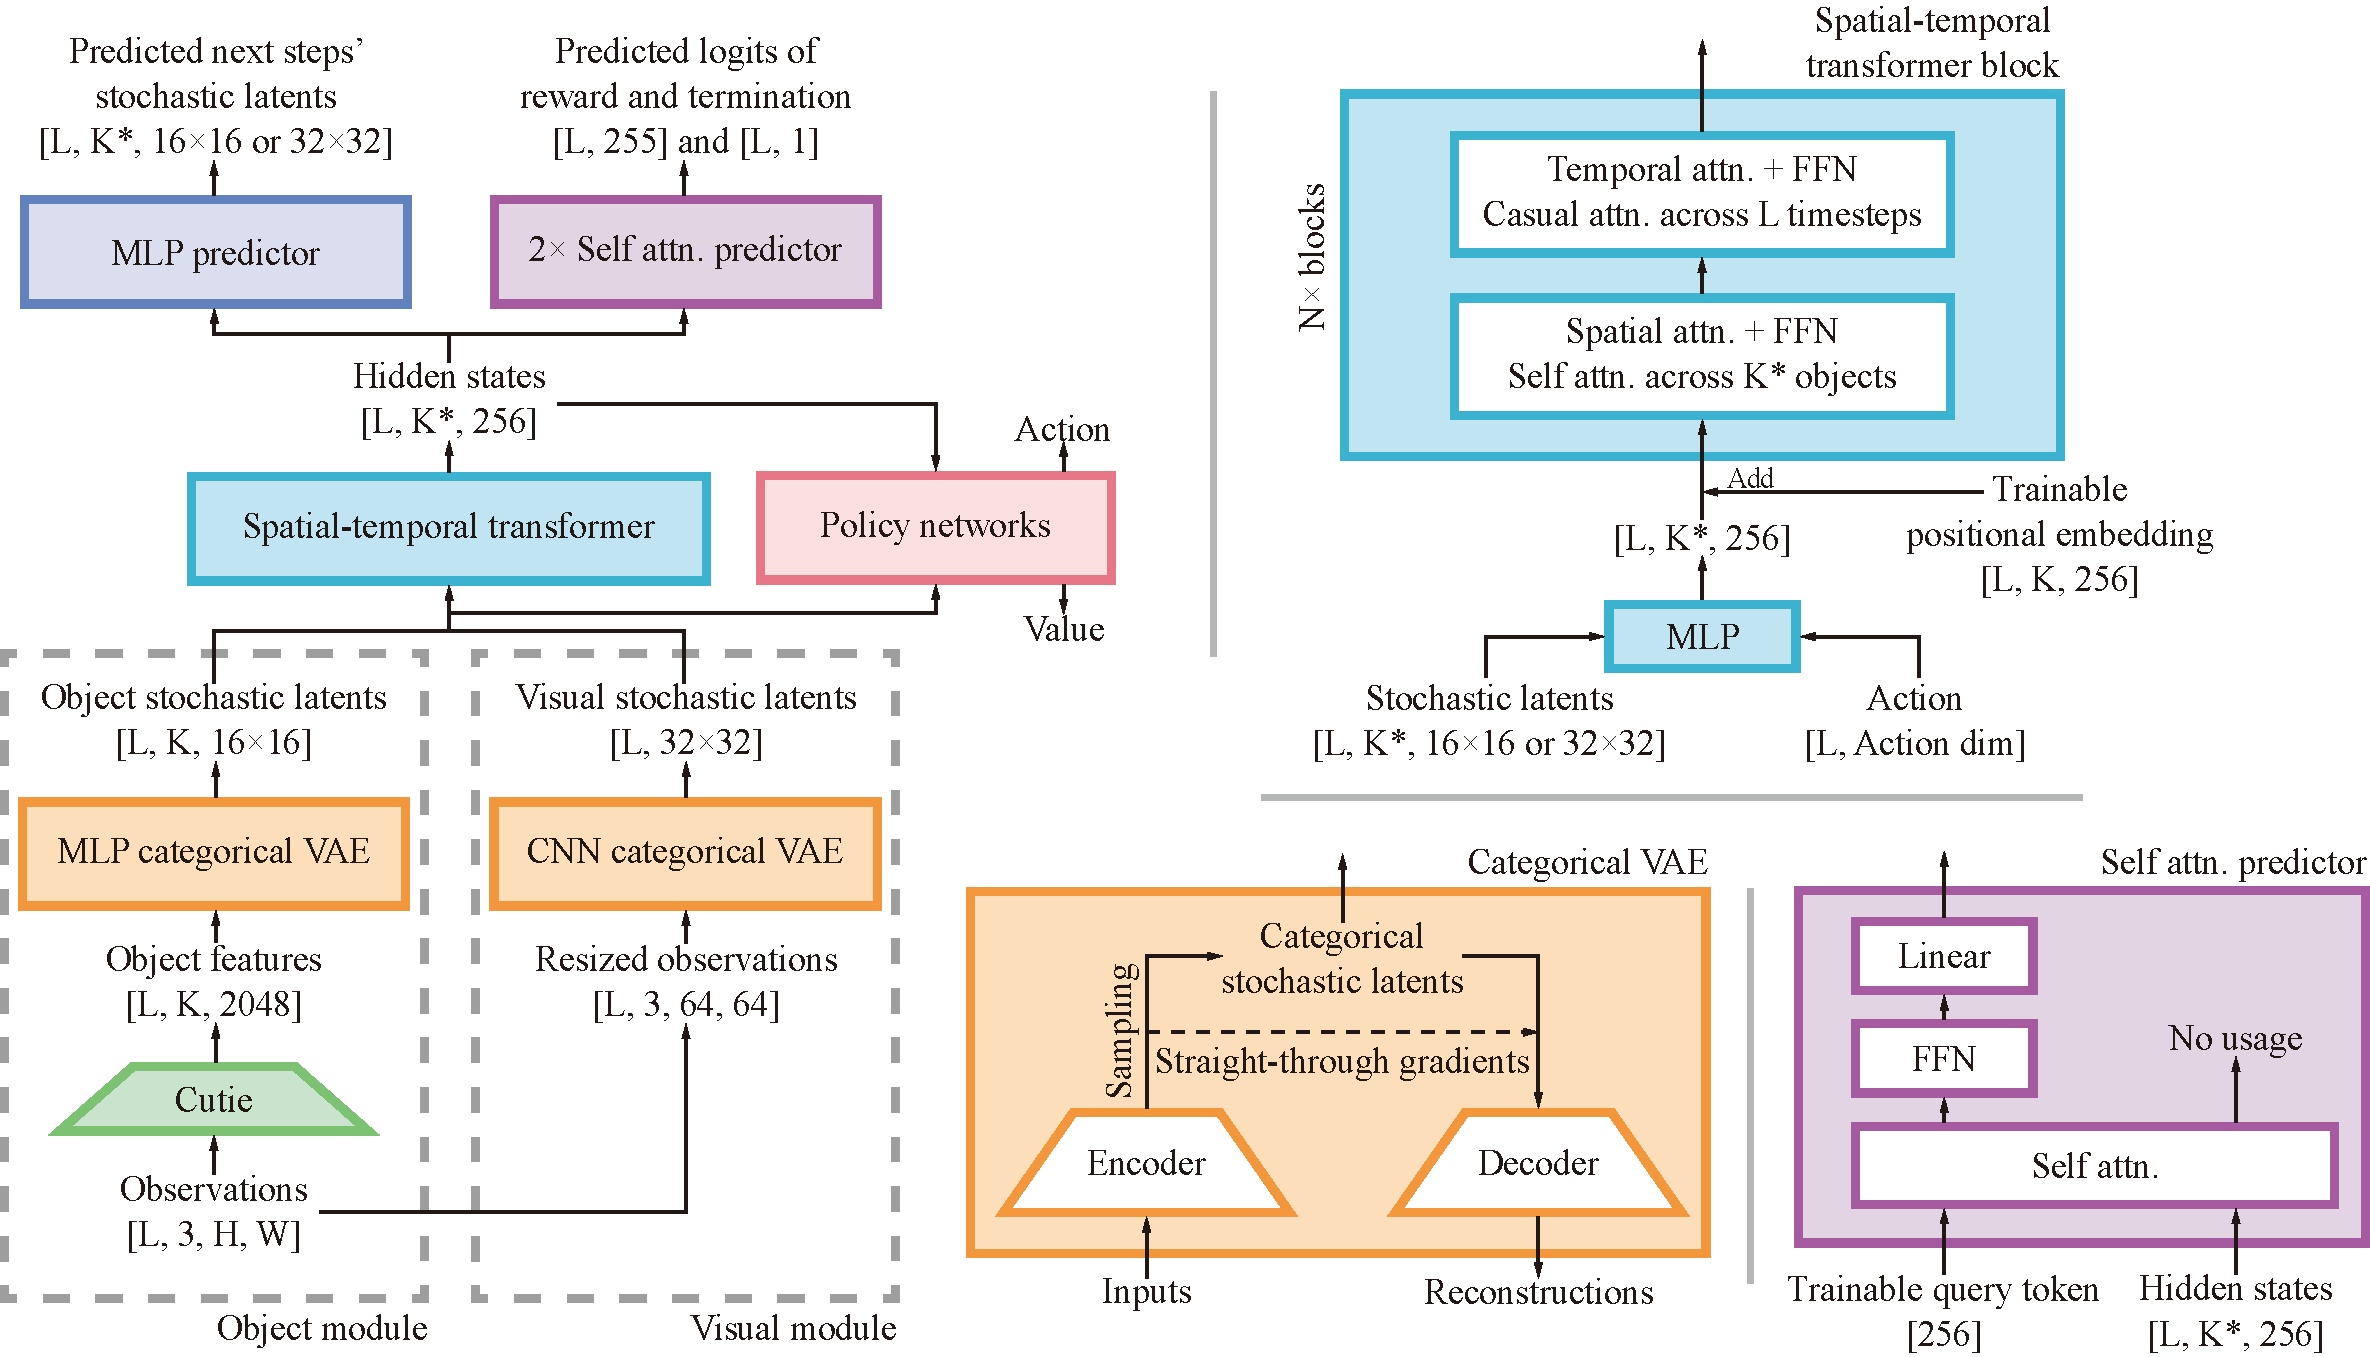
\includegraphics[width=0.8\textwidth]{figures/model-structure.pdf}
    \caption{
        The model structure of our proposed OC-STORM.
        The tuples in square brackets represent the shapes of the corresponding tensors, where $L$ denotes the batch length or sequence length, $K$ is the number of objects, and $H$ and $W$ are the image height and width, respectively.
        The object module constitutes the proposed object-centric component, while the visual module processes resized raw observations.
        $K^*$ equals $K$ when only object module is used, equals $1$ when only visual module is used, and equals $K+1$ when both modules are used.
        The trainable token and positional embeddings are broadcast to match the shapes of the corresponding tensors.
        The reward logit is 255-dimensional and used for the symlog two-hot loss \citep{hafner_mastering_2023}.
    }
    \label{fig:model-structure}
\end{figure*}

%%%%%%%%%%%%%%%%%%%%%%%%%%%%%%%%%%%%%%%%%%%%%%%%%%%%%%%%%%%%%%%%%%%%%%%%%%%%%%%%%%%%%%%%
% Optimize equations
%%%%%%%%%%%%%%%%%%%%%%%%%%%%%%%%%%%%%%%%%%%%%%%%%%%%%%%%%%%%%%%%%%%%%%%%%%%%%%%%%%%%%%%%
\section{Loss Functions} \label{sec:loss-func}

\subsection{World Model Learning}
The world model is trained in a self-supervised manner, optimizing it end-to-end.
Our setup closely follows DreamerV3 \citep{hafner_mastering_2023}, with details presented for completeness.
We use mean squared error (MSE) loss for reconstructing the original inputs, symlog two-hot loss $\mathcal{L}_{\rm sym}$ \citep{hafner_mastering_2023} for reward prediction, and binary cross-entropy (BCE) loss for termination signal prediction. 
These losses, collectively referred to as prediction loss, are defined as:
\begin{equation} \label{eq:pred_losses}
\mathcal{L}_{\rm pred}(\phi) = \underbrace{||\hat{s}_t - s_t||^2_2}_{\text{Reconstruction loss}} +
\underbrace{\mathcal{L}_{\rm sym}(\hat{r}_t, r_t)}_{\text{Reward loss}} +
\underbrace{\tau_t \log \hat{\tau}_t + (1 - \tau_t) \log (1 - \hat{\tau}_t)}_{\text{Termination loss}}.
\end{equation}

The dynamics loss $\mathcal{L}^{\rm dyn}_t(\phi)$ guides the sequence model in predicting the next distribution.
The representation loss $\mathcal{L}^{\rm rep}_t(\phi)$ allows the encoder’s output to be weakly influenced by the sequence model’s prediction, ensuring that the dynamics are not overly difficult to learn.
These losses are identical Kullback–Leibler (KL) divergence losses except for their gradient propagation settings.
We use $\mathrm{sg}(\cdot)$ to denote the stop gradient operation. The dynamics and representation losses are defined as:
\begin{subequations} \label{eq:dyn-losses}
\begin{alignat}{2}
\mathcal{L}_{\rm dyn}(\phi) &= \max\bigl(1, \mathrm{KL}\bigl[\mathrm{sg}(q_\phi(z_{t+1}|s_{t+1}))\ ||\  g^{\mathrm{dyn}}_\phi(\hat{z}_{t+1}|h_t) \bigr]\bigr), \label{eq:dyn_loss}\\
\mathcal{L}_{\rm rep}(\phi) &= \max\bigl(1, \mathrm{KL}\bigl[q_\phi(z_{t+1}|s_{t+1})\ ||\ \mathrm{sg}( g^{\mathrm{dyn}}_\phi(\hat{z}_{t+1}|h_t)) \bigr]\bigr).
\end{alignat}
\end{subequations}
The $\max$ operation represents free bits for KL divergence, encouraging the model to focus on optimizing prediction losses for better feature extraction if the KL divergence is too small.

The total loss function for training the world model is calculated as follows, where $\mathbb{E}_{\mathcal{D}}$ denotes the expectation over samples from the replay buffer:
\begin{equation} \label{eq:world_model_full_loss}
\mathcal{L}(\phi) = \mathbb{E}_{\mathcal{D}}\Bigl[\mathcal{L}_{\rm pred}(\phi) + \mathcal{L}_{\rm dyn}(\phi) + 0.5 \mathcal{L}_{\rm rep}(\phi)\Bigr].
\end{equation}
The coefficient of 0.5 for $\mathcal{L}_{\rm rep}$ is used to prevent posterior collapse \citep{lucas_understanding_2019}, a situation where the model produces the same distribution for different inputs, causing the dynamics loss to trivially converge to 0.
The imbalanced KL divergence loss helps to mitigate this issue.


\subsection{Policy Learning} \label{sec:policy-learning}
% multi dim action space
The policy learning approach closely follows that of DreamerV3 \citep{hafner_mastering_2023}, with modifications specific to our method.
The key differences lie in the input for the policy and the action dimension for the game Hollow Knight.
We use the concatenation of object latents, object hidden states, visual latents, and visual hidden states as input features.
For Hollow Knight, a multi-discrete action space is employed.

The agent learns entirely on the imagined trajectories generated by the world model.
To begin the imagination process, we first sample a short contextual trajectory from the replay buffer.
During imagination, future environmental inputs $s_{t+1:L}$ are unknown, and sampling from the posterior distribution $q_\phi(z_t|s_t)$ is unavailable.
Thus, we sample the latent variable from the prior distribution $g^{\mathrm{dyn}}_\phi(\hat{z}_{t+1}|h_t)$ and optimize the policy over $\hat{z}_{t+1}$.
However, during testing, the agent interacts directly with the environment, allowing access to the posterior distribution of the last observation.
This introduces a difference in notation.
For simplicity, we do not distinguish between $z_t$ and $\hat{z}_t$ in the following descriptions.

The agent uses both the latent variable $\hat{z}_{t}$ and hidden states $h_t$ as inputs, as defined below:
\begin{equation} \label{eq:agent}
\begin{aligned}
&\text{Critic:} & V_\psi(z_{t}, h_t)&\approx \mathbb{E}_{\pi_\theta, \phi}\Bigl[\sum_{k=0}^T \gamma^k r_{t+k}\Bigr],\\
&\text{Actor:} & a_t&\sim\pi_\theta(a_t|z_{t}, h_t).\\
\end{aligned}
\end{equation}
Here, $T$ is the number of timesteps in the episode. We use two separate MLPs for the critic and actor networks.
The symbol $\phi$ indicates that the trajectories are generated within the imagination process of the world model.

For value loss, we employ the $\lambda$-return $G^\lambda_{t}$ \citep{sutton_reinforcement_2018, hafner_mastering_2023} to improve value estimation.
It is recursively defined as follows, where $\hat{r}_t$ is the reward predicted by the world model, and $\hat{\tau}_t$ represents the predicted termination signal:
\begin{subequations}
    \label{eq:lambda-return}
    \begin{align}
        G^\lambda_{t} &\doteq \hat{r}_t + \gamma (1-\hat{\tau}_t) \Bigl[(1-\lambda) V_{\psi}(z_{t+1}, h_{t+1}) + \lambda G^{\lambda}_{t+1}\Bigr], \\
        G^\lambda_{L} &\doteq V_{\psi}(z_{L}, h_{L}).
    \end{align}
\end{subequations}

To regularize the value function, we maintain an exponential moving average (EMA) of the critic's parameters, as defined in Equation \eqref{eq:slow_critic}.
This regularization technique stabilizes training and helps prevent overfitting, where $\psi_t$ represents the current critic parameters, $\sigma$ is the decay rate, and $\psi^{\mathrm{EMA}}_{t+1}$ denotes the updated critic parameters:
\begin{equation} \label{eq:slow_critic}
\psi^{\mathrm{EMA}}_{t+1} = \sigma \psi^{\mathrm{EMA}}_t + (1-\sigma) \psi_{t}.
\end{equation}

For policy gradient loss, we apply return-based normalization for the advantage value.
The normalization ratio $S$ is defined in Equation \eqref{eq:norm-ratio} as the range between the 95th and 5th percentiles of the $\lambda$-return $G^\lambda_{t}$ across the batch \citep{hafner_mastering_2023}:
\begin{equation} \label{eq:norm-ratio}
\begin{gathered}
S = \mathrm{percentile}(G^\lambda_{t}, 95) - \mathrm{percentile}(G^\lambda_{t}, 5).\\
\end{gathered}
\end{equation}

The complete loss functions for the actor-critic algorithm are given by Equation \eqref{eq:reinforce}:
\begin{subequations} \label{eq:reinforce}
\begin{align}
\label{eq:reinforce_actor}
\mathcal{L}(\theta)& = \mathbb{E}_{\pi_\theta, \phi}\biggl[-\mathrm{sg}\bigg(\frac{G^\lambda_{t}- V_{\psi}(s_{t})}{\max(1, S)}\bigg) \ln \pi_\theta(a_t|z_t, h_t) -\eta H\bigl(\pi_\theta(a_t|z_t, h_t)\bigr)\biggr],\\
\label{eq:reinforce_critic}
\mathcal{L}(\psi)& =  \mathbb{E}_{\pi_\theta, \phi}\biggl[
\mathcal{L}_{\rm sym}\Bigl(V_\psi(z_t, h_t), \mathrm{sg}\bigl(G^\lambda_{t}\bigr)\Bigr) +
\mathcal{L}_{\rm sym}\Bigl(V_\psi(z_t, h_t), \mathrm{sg}\bigl(V_{\psi^{\mathrm{EMA}}}(z_t, h_t)\bigr)\Bigr)\biggr].
\end{align}
\end{subequations}
Here, $H(\cdot)$ denotes the entropy of the policy distribution, and $\eta=1\times 10^{-3}$ is the coefficient for entropy loss.

\newpage
\section{Comparison With other MBRL Algorithms} \label{sec:full-compare}

\begin{table*}[h]  
  \caption{Game scores, overall human-normalized scores, and computing time on the Atari $100$k benchmark. Bold indicates scores within 5\% of best. The last column `\#obj' denotes manually annotated objects per game.
  The DreamerV3 scores here are the original data from their paper \citep{hafner_mastering_2023}.
  SPR \citep{schwarzer_data-efficient_2021} is a typical sample-efficient model-free method.
  IRIS \citep{micheli_transformers_2022} and TWM \citep{robine_transformer-based_2022} are transformer-based MBRL approaches, and $\Delta$-IRIS \citep{micheli_efficient_2024} is an upgraded version.
  DIAMOND \citep{alonso_diffusion_2024} is a diffusion-based MBRL approach.
  }
  \label{table:atari-100k-comparisons}
  \centering
  \resizebox{1.0\textwidth}{!}{\begin{tabular}{lrr|rrrrrrr}
    \toprule
    Game & Random & Human & SPR & IRIS & TWM & DreamerV3 & $\Delta$-IRIS & DIAMOND & OC-STORM \\
    \midrule
    Alien & 228 & 7128 & 842 & 420 & 675 & \textbf{1278} & 599 & 744 & 1101\\
    Amidar & 6 & 1720 & 180 & 143 & 122 & 120 & 51 & \textbf{226} & 163\\
    Assault & 222 & 742 & 566 & \textbf{1524} & 683 & 741 & 1435 & \textbf{1526} & 1270\\
    Asterix & 210 & 8503 & 962 & 854 & 1117 & 1020 & 2001 & \textbf{3698} & 1754\\
    BankHeist & 14 & 753 & 345 & 53 & 467 & 422 & \textbf{1206} & 20 & 1075\\
    BattleZone & 2360 & 37188 & 14834 & 13074 & 5068 & \textbf{20800} & 10365 & 4702 & 4590\\
    Boxing & 0 & 12 & 36 & 70 & 78 & 87 & 56 & 87 & \textbf{92}\\
    Breakout & 2 & 30 & 20 & 84 & 20 & 11 & \textbf{226} & 132 & 52\\
    ChopperCommand & 811 & 7388 & 946 & 1565 & 1697 & \textbf{2440} & 1101 & 1370 & 2090\\
    CrazyClimber & 10780 & 35829 & 36700 & 59324 & 71820 & 80060 & 70920 & \textbf{99168} & 84111\\
    DemonAttack & 152 & 1971 & 518 & \textbf{2034} & 350 & 454 & 884 & 288 & 411\\
    Freeway & 0 & 30 & 19 & 31 & 24 & 0 & 31 & 33 & 0\\
    Frostbite & 65 & 4335 & 1171 & 259 & 1476 & \textbf{3914} & 287 & 274 & 260\\
    Gopher & 258 & 2412 & 661 & 2236 & 1675 & 2252 & \textbf{9349} & 5898 & 4457\\
    Hero & 1027 & 30826 & 5859 & 7037 & 7254 & \textbf{13324} & 6235 & 5622 & 6441\\
    Jamesbond & 29 & 303 & 366 & 463 & 362 & \textbf{490} & 345 & 427 & 347\\
    Kangaroo & 52 & 3035 & 3617 & 838 & 1240 & 2840 & 1573 & \textbf{5382} & 4218\\
    Krull & 1598 & 2666 & 3682 & 6616 & 6349 & 8604 & 6392 & 8610 & \textbf{9715}\\
    KungFuMaster & 258 & 22736 & 14783 & 21760 & \textbf{24555} & \textbf{25560} & \textbf{25159} & 18714 & \textbf{24988}\\
    MsPacman & 307 & 6952 & 1318 & 999 & 1588 & 1400 & 1175 & 1958 & \textbf{2401}\\
    Pong & -21 & 15 & -5 & 15 & 19 & -5 & 15 & \textbf{20} & \textbf{21}\\
    PrivateEye & 25 & 69571 & 86 & 100 & 87 & \textbf{3238} & 100 & 114 & 85\\
    Qbert & 164 & 13455 & 866 & 746 & 3331 & 3700 & 3438 & \textbf{4499} & \textbf{4546}\\
    RoadRunner & 12 & 7845 & 12213 & 9615 & 9109 & 18440 & 10622 & \textbf{20673} & \textbf{20482}\\
    Seaquest & 68 & 42055 & 558 & 661 & 774 & \textbf{964} & 895 & 551 & 712\\
    UpNDown & 533 & 11693 & 10859 & 3546 & 15982 & \textbf{49456} & 8091 & 3856 & 6623\\
    \midrule
    HNS mean & 0\% & 100\%  & 61.6\% & 104.6\% & 95.6\% & 128.2\% & 138.3\% & \textbf{145.9\%} & 134.8\% \\ 
    HNS median & 0\% & 100\%  & 39.6\% & 28.9\% & 50.5\% & 48.7\% & \textbf{59.4\%} & 37.3\% & 43.8\% \\
    \midrule
    \makecell[bl]{Average compute\\4090 GPU days} & & & \makecell[br]{PyTorch\\0.1} & \makecell[br]{PyTorch\\3.5} & \makecell[br]{PyTorch\\0.4} & \makecell[br]{Jax\\0.1} & \makecell[br]{PyTorch\\1.0} & \makecell[br]{PyTorch\\2.9} & \makecell[br]{PyTorch\\0.2}\\
    \bottomrule
    \end{tabular}}
\end{table*}

%%%%%%%%%%%%%%%%%%%%%%%%%%%%%%%%%%%%%%%%%%%%%%%%%%%%%%%%%%%%%%%%%%%%%%%%%%%%%%%%%%%%%%%%
% Review
%%%%%%%%%%%%%%%%%%%%%%%%%%%%%%%%%%%%%%%%%%%%%%%%%%%%%%%%%%%%%%%%%%%%%%%%%%%%%%%%%%%%%%%%
\newpage
\section{Review of Object Representation Methods} \label{sec:review-segmentation}
\begin{table}[h]
  \caption{A brief review of state-of-the-art methods in different fields of computer vision related to object-centric reinforcement learning.}
  \label{table:review-segmentation}
  \centering
  \resizebox{1.0\textwidth}{!}{
    \begin{tabular}{p{0.2\textwidth}p{0.8\textwidth}}
        \toprule
        \textbf{Method} & \textbf{Description} \\
        \midrule
        Cutie & Retrieval-based semi-supervised video object segmentation algorithm.
        Provides compact vector representation of objects using an object transformer \citep{cheng_putting_2023}.\\
        \hline
        XMem & Retrieval-based semi-supervised video object segmentation algorithm with multi-level memory system.
        Lacks compact object representation \citep{cheng_xmem_2022}.\\
        \hline
        SAM & Open-set image segmentation algorithm.
        Generates masks via user prompts but requires a prompt for each frame in a video \citep{kirillov_segment_2023}.\\
        \hline
        TrackAnything & SAM + XMem for fine-grained video segmentation.
        Requires twice the computational resources compared to XMem \citep{yang_track_2023}.\\
        \hline
        PerSAM & One-shot enhancement of SAM. Difficult to expand to few-shot cases \citep{zhang_personalize_2023}.\\
        \hline
        SAM2 & State-of-the-art multi-usage video object segmentation algorithm.
        Capable of providing compact vector representations. \citep{ravi_sam_2024}.
        \\
        \hline
        YOLO & Closed-set object detection algorithm.
        Requires extensive annotations for training or fine-tuning \citep{redmon_you_2016, jocher_ultralytics_2023}.\\
        \hline
        GroundingDINO & Open-set object detection algorithm.
        Generates object bounding boxes using natural language prompts but struggles with rare or abstract cases, such as video game players \citep{liu_grounding_2023}.\\
        \hline
        Slot attention & Unsupervised image object discovery and segmentation algorithm.
        Underperforms compared to supervised methods \citep{locatello_object-centric_2020}. \\
        \hline
        SAVi & Unsupervised video object discovery and segmentation algorithm.
        Evaluation is semi-supervised, though training is unsupervised. Underperforms compared to semi-supervised methods \citep{kipf_conditional_2022, elsayed_savi_2022}. \\
        \hline
        Omnimotion & Video point-tracking algorithm.
        Provides pixel-level tracking but lacks object-level information and does not support few-shot scenarios \citep{wang_tracking_2023}.\\
        \hline
        Unimatch & Dense optical flow and depth estimation algorithm.
        Useful for moving identity detection but cannot extract object-level information and struggles with out-of-domain generalization \citep{xu_unifying_2023}.\\
        \bottomrule
    \end{tabular}
  }
\end{table}

%%%%%%%%%%%%%%%%%%%%%%%%%%%%%%%%%%%%%%%%%%%%%%%%%%%%%%%%%%%%%%%%%%%%%%%%%%%%%%%%%%%%%%%%
% Hollow Knight
%%%%%%%%%%%%%%%%%%%%%%%%%%%%%%%%%%%%%%%%%%%%%%%%%%%%%%%%%%%%%%%%%%%%%%%%%%%%%%%%%%%%%%%%
\section{Hollow Knight}
\subsection{Numerical Results} \label{sec:hollow-knight-numerical-results}

\begin{table*}[h]  
  \caption{
    Episode returns and win rates (WR) of STORM and the proposed OC-STORM on Hollow Knight.
    Each seed's performance is measured by the mean episode return across $20$ runs, and the average of these 3 mean returns is reported.
    The ``\#obj" column shows the number of annotated objects for a boss.
    Scores that are the highest or within $5\%$ of the highest score are highlighted in bold.
    To evaluate the upper limit of our agent, we conduct a 400k run on Pure Vessel, which demonstrates that our agent can defeat one of the most difficult bosses in the game with sufficient training.
  }
  \label{table:hollow-knight-results}
  \centering
  \resizebox{0.9\textwidth}{!}{\begin{tabular}{lrr|rr|rr|c}
    \toprule
    Boss name & Random & Optimal & STORM & OC-STORM & STORM WR & OC-STORM WR & \#obj\\
    \midrule
    God Tamer        & 10 & 56 & 35.0  & \textbf{41.7} & \textbf{70.0\%} & 55.0\%  & 4\\
    Hornet Protector & 7  & 37 & 28.1  & \textbf{32.4} & 66.7\%  & \textbf{100.0\%} & 2 \\
    Mage Lord        & 3  & 38 & 19.6  & \textbf{28.0} & 5.0\% & \textbf{48.0\%} & 3  \\
    Mantis Lords     & 2  & 42 & 33.2  & \textbf{35.2} & 71.7\% & \textbf{83.3\%} & 3  \\
    Mawlek           & 8  & 41 & \textbf{36.9}  & \textbf{37.2} & \textbf{98.3\%} & \textbf{98.3\%}  &  3\\
    Pure Vessel      & 2  & 55 & 8.9   & \textbf{15.7} & 0.0\% & 0.0\%  & 2 \\
    Pure Vessel (400k)&2  & 55 & 25.3  & \textbf{35.0} & 6.7\% & \textbf{13.3\%} & 2 \\
    \bottomrule
  \end{tabular}}
\end{table*}

\subsection{Related Work} \label{sec:hollow-knight-review}
Despite its popularity among players, Hollow Knight has seen limited use as a benchmark for research in reinforcement learning.
We introduce repositories, published research, and other relevant resources that leverage or explore Hollow Knight as a benchmark.
\citet{cui_ailec0623dqn_hollowknight_2021} employs DQN \citep{mnih_human-level_2015} and its variants but requires modding the game background to black to enhance character perception.
\citet{yang_seermerhollowknight_rl_2023} uses the Rainbow algorithm \citep{hessel_rainbow_2017} with additional techniques like DrQ \citep{yarats_mastering_2021, kostrikov_image_2021}, achieving high win rates against several of the game’s bosses.
Yang's repository has been widely forked and adopted.
Building on his work, \citet{lee_adapting_2023} studies the effect of reward shaping, while \citet{sun_moapacharl-hollowknight-zote_2024} focuses on improving training efficiency by tuning the game interaction configuration and switching to the PPO algorithm \citep{schulman_proximal_2017}.
\citet{jain_adityajain1030hkrl_2024} leverages internal game states to extract hitboxes as input for the algorithm, representing them as segmentation masks that are passed to DQN or PPO.

\subsection{Environment Configuration} \label{sec:HK-exp-dev}
Hollow Knight is a modern video game developed with Unity \citep{unity_2005}. 
To our knowledge, efficient simulators for this game, such as those available for Atari \citep{brockman_openai_2016, towers_gymnasium_2023}, are not publicly available. 
Therefore, we developed a custom wrapper that captures screenshots of the game at 9 FPS and sends keyboard signals to execute actions.
The 9 FPS rate is a choice based on the author's experience with the game and considerations for computational efficiency.
To obtain reward signals, we developed a modding plugin \citep{hk-moddingapi_2017} that logs when the player-controlled character (the Knight) either hits an enemy or is hit. 
Our wrapper then parses this log file to generate reward and termination signals.

The game execution and agent training are conducted on a Windows machine. 
To monitor training progress and statistics without interrupting the game, we needed a method to send keyboard inputs to a background or unfocused window. 
However, Windows lacks an API for this purpose.
As a result, the game window must remain in the foreground, fully occupying the training device and hindering monitoring.
To address this, we utilized a Hyper-V \citep{scooley_introduction_2022} Windows virtual machine to run the game in the background, with Ray \citep{moritz_ray_2018} facilitating communication between the host and virtual machine. 
Training and processing occur on the host machine, while the virtual machine handles interactions with the environment. 
This setup can be extended to distributed nodes, with some handling game rendering and others managing training tasks.

For in-game configuration, the charms \citep{fandom_categorycharms_2018} are set to Unbreakable Strength, Quick Slash, Soul Catcher, and Shaman Stone across all experiments. 
This configuration is chosen to explore the agent's fighting potential rather than its glitch-finding abilities.

\subsection{Action Space} \label{sec:hk-action-space}
All previous works utilize a human-specified action space rather than the original keyboard inputs.
For example, in the \citet{yang_seermerhollowknight_rl_2023} implementation, short and long jumps are treated as two distinct actions, which are originally controlled by the duration of the jump button press.
His environment wrapper handles this difference with a fixed command.
While this design reduces the exploration and computational costs for reinforcement learning agents, it cannot capture the full range of possible actions in the game.
Advanced operations, as demonstrated in this video \citep{crankytemplar_hollow_2018}, require full control of the keyboard.
Therefore, we design the action space as a multi-binary-discrete one that directly binds to the press and release of the physical keyboard, which will be explained in Section \ref{sec:hk-action-space}.

We design the action space as a multi-binary-discrete space directly mapped to the press and release states of eight specific keys on the keyboard.
These keys include \texttt{W}, \texttt{A}, \texttt{S}, and \texttt{D} for movement directions, and \texttt{J}, \texttt{K}, \texttt{L}, and \texttt{I} for attack, jump, dash, and spell actions, respectively.
Each key's state is represented as a binary variable, where 0 corresponds to a key release and 1 corresponds to a key press.
The action can therefore be described as $a \in \{0, 1\}^8$, with each element representing the binary state of one key.
The key's state is maintained between frames, and a toggle signal is sent only when there is a change in the key state from $0 \rightarrow 1$ (press) or $1 \rightarrow 0$ (release).

The probability of an action is determined by the independent probabilities of each key's state:
\begin{equation}
    \pi_\theta(a|z, h) = \prod_{k=1}^{8} \pi_\theta(a^k|z, h)
\end{equation}
where $a^k$ denotes the state of the $k$-th key.

The entropy of the action space, $H(\pi_\theta(a|z, h))$, is the sum of the entropies of the individual key states:
\begin{equation}
    H(\pi_\theta(a|z, h)) = \sum_{k=1}^{8} H(\pi_\theta(a^k|z, h))
\end{equation}

This design provides fine-grained control over the agent's actions, allowing for the execution of complex manoeuvres while maintaining a tractable exploration space for reinforcement learning.

\subsection{Reward Shaping in Hollow Knight} \label{sec:reward-shaping}
Most existing methods \citep{yang_seermerhollowknight_rl_2023, sun_moapacharl-hollowknight-zote_2024, jain_adityajain1030hkrl_2024, cui_ailec0623dqn_hollowknight_2021, lee_adapting_2023} for Hollow Knight use a reward structure of +1 for hitting an enemy and -1 for taking damage.
Some approaches modify the weighting ratios, while others introduce auxiliary rewards for performing specific actions.
However, we found that these settings are suboptimal for training reinforcement learning agents.

Our method assigns a +1 reward signal for hitting an enemy and a virtual termination signal upon being hit.
The game continues until the episode naturally ends. 
The termination signal is stored in the replay buffer for training the world model, treating health loss as a life-loss event. 
Leveraging life-loss information is a common technique that aids in value estimation \citep{ye_mastering_2021, micheli_transformers_2022, zhang_storm_2023, alonso_diffusion_2024}.
Additionally, the Knight can damage enemies in multiple ways, and these damages are normalized against the base attack damage to compute the positive reward.


\begin{figure}[h]
    \centering
    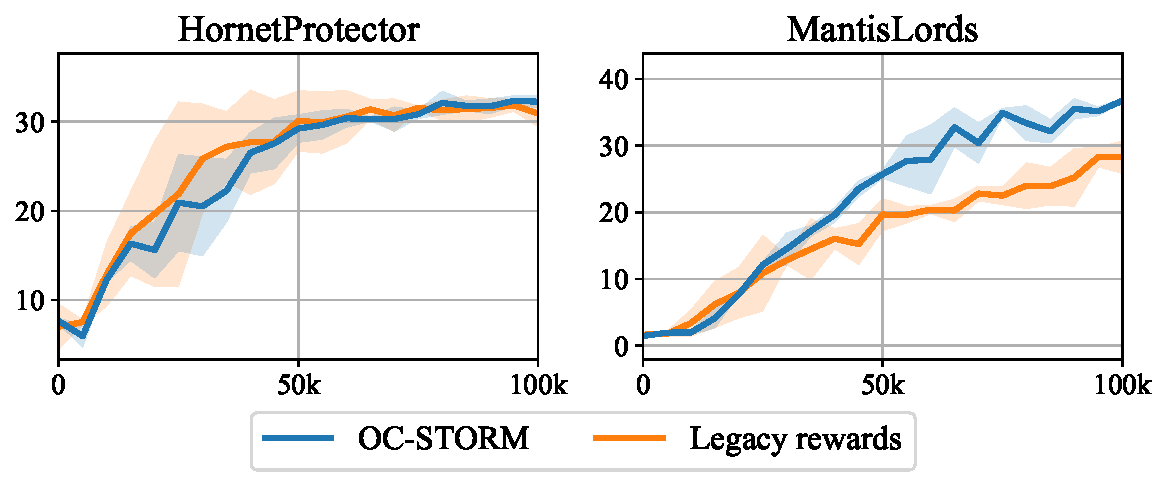
\includegraphics[width=0.5\textwidth]{figures/reward-shaping-ablation.pdf}
    \caption{
        Training episode returns for Hollow Knight's Hornet Protector and Mantis Lords under different reward settings.
        ``Legacy rewards" refer to the reward scheme used in prior works.
        For comparison, we aligned the returns from "legacy rewards" with our baseline settings by accounting for lost health.
    }
    \label{fig:reward-ablation}
\end{figure}

Here, we present the key differences between the two reward settings.
As illustrated in Figure \ref{fig:reward-ablation}, our reward configuration is more robust than those used in previous studies, resulting in significantly improved performance, especially in more challenging environments like Mantis Lords.
This improvement can be analyzed from two perspectives:
\begin{enumerate}
    \item Terminating the episode upon being hit better aligns with human cognition and the agent's expected behaviour.
    The aim is for the agent to deal as much damage as possible without taking any.
    While this may seem aggressive, raising concerns that the agent might sacrifice itself to deal more damage, neither our qualitative nor quantitative results show this tendency.
    Survival naturally offers more opportunities to deal with future damage, which the agent learns to prioritize.
    Although applying a negative penalty for being hit could prevent the agent from sustaining multiple consecutive hits in highly unfavourable situations, such scenarios should not occur under an optimal or near-optimal policy.
    \item While maintaining the same optimal policy, truncating future rewards upon being hit significantly reduces the variance in value estimation.
    Hollow Knight is a highly stochastic environment where bosses behave aggressively yet unpredictably.
    Estimating value directly over an episode (lasting approximately 300 to 700 timesteps) is inherently challenging in such settings.
\end{enumerate}


\subsection{Comparison with a Model-Free Baseline} \label{sec:model-free-comparison}

As introduced in Section \ref{sec:hollow-knight-review}, Yang's repository \citep{yang_seermerhollowknight_rl_2023} is a widely recognized implementation within the community.
In this section, we compare the performance against the boss Hornet Protector.

Yang's reward structure assigns +0.8 for hitting an enemy and -0.8 for taking damage, with additional auxiliary rewards on the order of $1 \times 10^{-4}$ for various actions. A small feedback reward is also given at the end of each episode. 
The choice of a 0.8 weight factor for rewards reflects the use of +1/-1 reward clipping, with a margin reserved for the auxiliary rewards.
We provide a broad comparison with this approach below.

\begin{figure}[h]
    \centering
    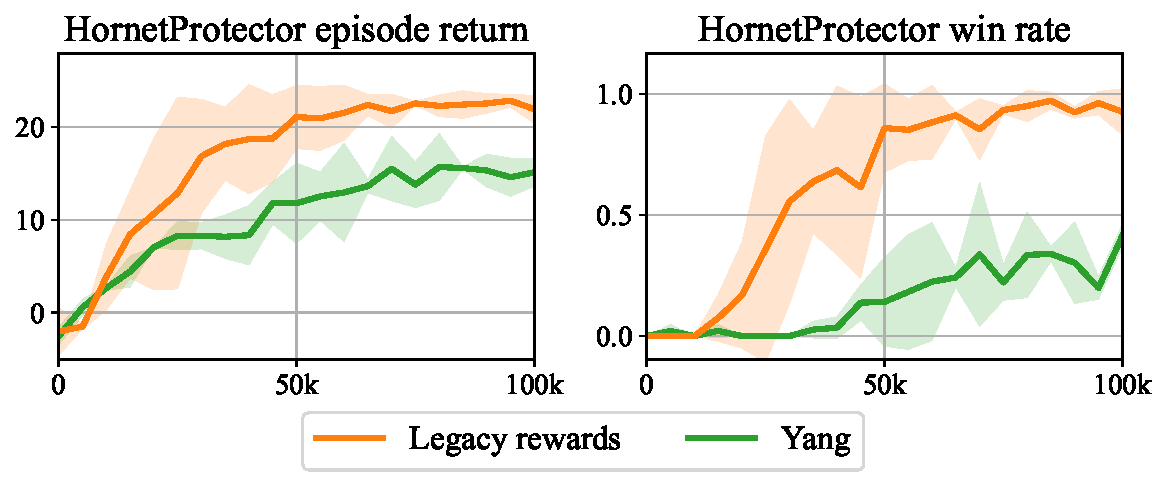
\includegraphics[width=0.5\textwidth]{figures/model-free-comparison.pdf}
    \caption{
        Training episode returns and win rates on Hollow Knight's Hornet Protector with our proposed method and Yang's \citep{yang_seermerhollowknight_rl_2023} method.
        ``Legacy rewards" are as described in Section \ref{sec:reward-shaping}.
        We applied some preprocessing to align the two returns for easier comparison, so the ``legacy rewards" curve may appear different from the one shown in the previous section.
        The win rate is more straightforward and can be used for comparison without changing.
    }
    \label{fig:model-free-comparison}
\end{figure}

As shown in Figure \ref{fig:model-free-comparison}, our implementation is more efficient than Yang's.
As we noted in Section \ref{sec:hollow-knight-results}, there are significant differences between our methods, making this \textbf{not strictly} a fair comparison from an algorithmic standpoint.
This comparison is intended solely to demonstrate the efficiency of our implementation.

Additionally, Yang claims that his agent can achieve 10 wins out of 10 battles, which is accurate despite his win rate in our plot appearing to be lower than 100\%. 
Two reasons may lead to this.
First, his original sample steps are greater than ours, which may account for differences in performance.
Second, our in-game charm configuration \citep{fandom_categorycharms_2018} differs from the one used in his implementation.
When testing Yang's implementation, we retained our current charm settings, which likely impacted the win rate results.

\newpage
\section{Additional and Analysis} \label{sec:additional-analysis}

%%%%%%%%%%%%%%%%%%%%%%%%%%%%%%%%%%%%%%%%%%%%%%%%%%%%%%%%%%%%%%%%%%%%%%%%%%%%%%%%%%%%%%%%
% Attention-based policy or MLP-based policy
%%%%%%%%%%%%%%%%%%%%%%%%%%%%%%%%%%%%%%%%%%%%%%%%%%%%%%%%%%%%%%%%%%%%%%%%%%%%%%%%%%%%%%%%
\subsection{Attention-Based policy or MLP-based Policy} \label{sec:attn-mlp-policy}
When handling multiple objects, an attention-based policy network like the self-attention predictor described in Appendix~\ref{sec:model-structure} is a natural choice.
A previous work OC-SA \citep{stanic_learning_2022} has also explored such structure.
However, we still design our actor and critic networks as MLPs which take the concatenation of object latent variables and hidden states as input.

We found that the attention-based policy tends to overfit pre-learned behaviours and makes it hard to learn new knowledge.
This will not be a major issue in stationary games like Boxing but will face trouble in non-stationary games like Pong.
For example, the attention-based policy can quickly learn how to catch the ball but cannot efficiently learn how to score against the opponent.
On the one hand, we can confirm this by visually checking the rendered episodes.
On the other hand, numerically speaking, we can observe the episode length of playing Pong.
If the episode length increases while the episode returns remain at the same level, then we can tell that the agent learns how to catch the ball, but is stuck in that local optimum.

\begin{figure}[h]
    \centering
    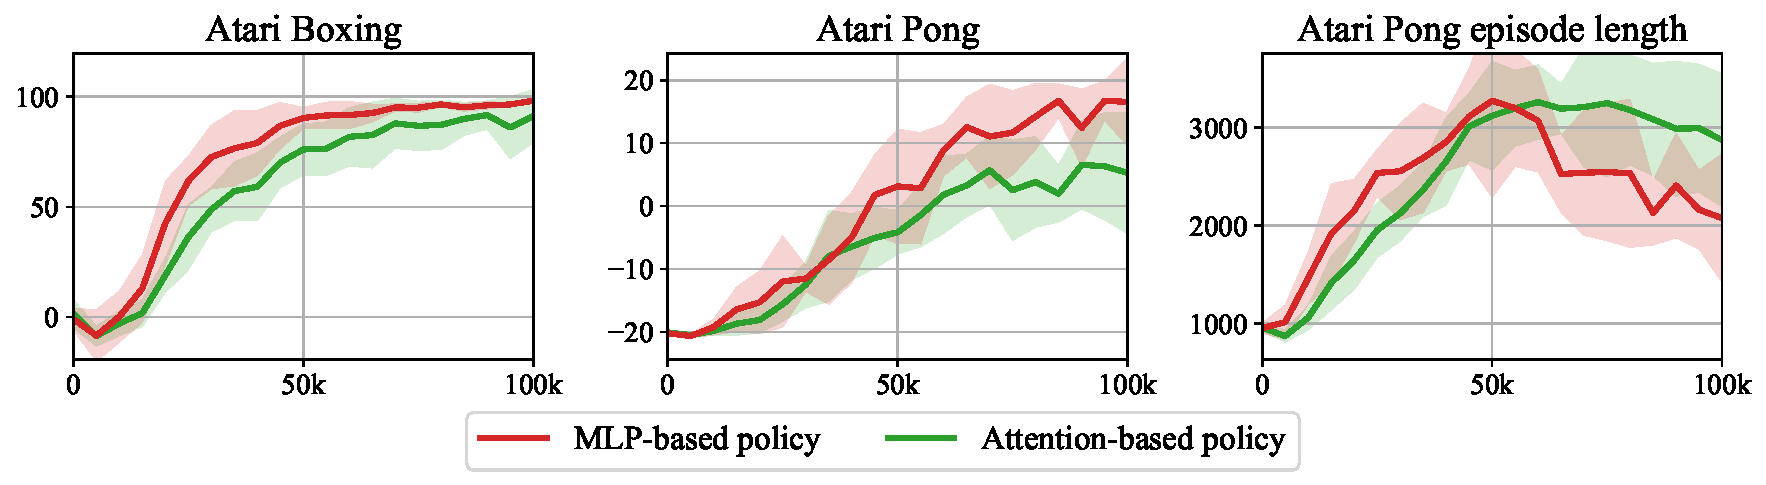
\includegraphics[width=0.75\textwidth]{figures/policy-ablation.pdf}
    \caption{
        Training episode returns for Atari Boxing, Pong and episode lengths for Pong of attention-based policy and MLP-based policy.
        The attention-based policy can learn as quickly as the MLP-based policy for catching the ball but struggles to transition to the scoring phase in Atari Pong.
    }
    \label{fig:policy-ablation}
\end{figure}

As the results plotted in Figure \ref{fig:policy-ablation}, we can tell that the attention-based policy suffers from that issue.
The episode length of both policies rises at a similar speed before 50k steps, but it declines slower for the attention-based policy after that.
The experiments are conducted using only the object module, so the MLP-based policy curves are identical to the ``vector" ones in Figure \ref{fig:module-ablation}.
As the visual latent itself contains all the information, the agent can choose only to use that part of the information and thus may affect our judgement on the effectiveness of the attention-based policy.

Though the attention-based policy has the potential to handle a dynamic number of objects, our experiments are conducted on a fixed number. 
As it doesn't demonstrate superior performance than the MLP-based policy in our case, we always use MLP-based in other tasks for consistency in evaluation.


%%%%%%%%%%%%%%%%%%%%%%%%%%%%%%%%%%%%%%%%%%%%%%%%%%%%%%%%%%%%%%%%%%%%%%%%%%%%%%%%%%%%%%%%
% Impact of the number of labelled images
%%%%%%%%%%%%%%%%%%%%%%%%%%%%%%%%%%%%%%%%%%%%%%%%%%%%%%%%%%%%%%%%%%%%%%%%%%%%%%%%%%%%%%%%
\subsection{Impact of the Number of Annotations} \label{sec:1shot}
% one more hornet if possible
Since Cutie is a retrieval-based algorithm that stores past frames and masks in a buffer for reference, it naturally supports the use of multiple annotation masks beyond the first frame by substituting model-generated masks in the buffer. 
Incorporating more label masks can capture a wider range of object states, leading to more consistent segmentation results.
However, reducing the number of labels can further lower annotation costs and computational complexity.
In this section, we explore the impact of the number of labels on agent performance.
To eliminate the influence of visual input, we conduct these experiments using only the object module.

\begin{figure}[h]
    \centering
    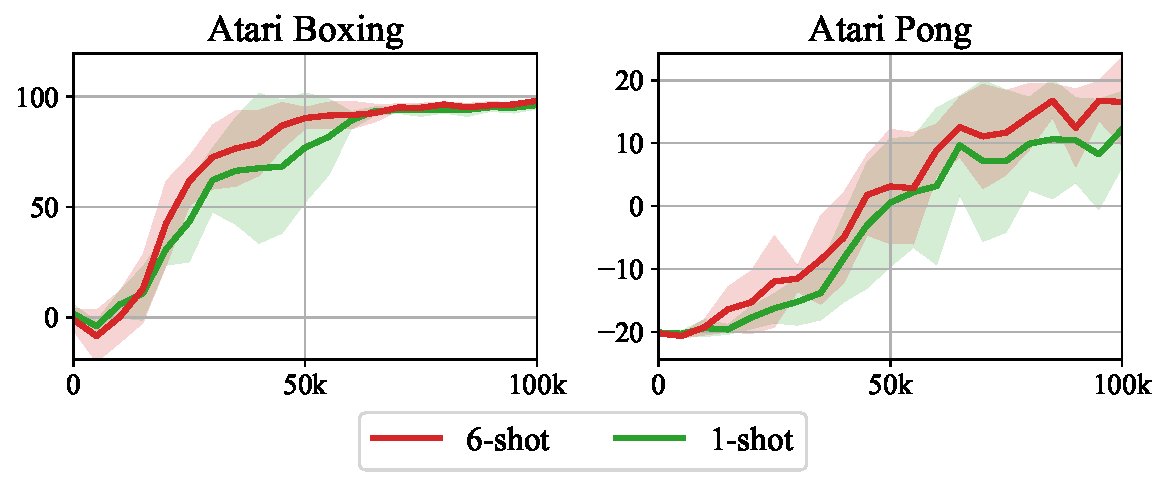
\includegraphics[width=0.5\textwidth]{figures/1shot-ablation.pdf}
    \caption{
        Training episode returns for Atari Boxing and Pong with different numbers of annotation segmentation masks.
        Increasing the number of annotation masks enhances the robustness of the agent's performance.
    }
    \label{fig:1shot-ablation}
\end{figure}

As shown in Figure \ref{fig:1shot-ablation}, increasing the number of annotation segmentation masks enhances the robustness of the agent's performance, even in visually static environments like Atari Boxing and Pong.
In these environments, a single frame can include all necessary objects for decision-making.
However, Cutie may lose track of objects if their states deviate significantly from those in the labelled masks, such as the punching state versus the standing state in Boxing, or the paddle in Pong when it is partially off-screen and appears shorter than when centred.

Moreover, in complex environments like Hollow Knight and Minecraft, a single frame may not capture all objects, which often necessitates additional segmentation masks.
For consistency in evaluation, we use six annotation segmentation masks for Atari and twelve for Hollow Knight.

\subsection{The Computational Overhead of OC-STORM}
The computational overhead of OC-STORM on Atari games with an NVIDIA GeForce RTX 3090 is shown in Table \ref{table:computational-overhead}.
The input resolution for Cutie is $420\times 320$ (double the original $210\times 160$).
Thus the computational cost of introducing Cutie is acceptable in many cases.

\begin{table}[h]  
  \caption{
    The computational overhead of OC-STORM on Atari games.
    The three numbers in a block here mean sample or evaluation speed (iterations/second), training speed (iterations/second) and hours spent for a train with a 100k sample budget, respectively.
  }
  \label{table:computational-overhead}
  \centering
  \resizebox{1.0\textwidth}{!}{\begin{tabular}{l|rrr|rrr|rrr|rrr}
    \toprule
    Algorithm & \multicolumn{3}{|c|}{0 objects} & \multicolumn{3}{|c|}{1 object} & \multicolumn{3}{|c|}{2 objects} & \multicolumn{3}{|c}{3 objects}\\
    \midrule
    \makecell[tl]{STORM \\ (visual module only)} & 114 it/s & 8.1 it/s & 3.67 h & \multicolumn{3}{|c|}{-} & \multicolumn{3}{|c|}{-} & \multicolumn{3}{|c}{-} \\
    \makecell[tl]{OC-STORM \\ (obj module only)} & \multicolumn{3}{|c|}{-} & 32 it/s & 8.8 it/s & 4.02 h & 32 it/s & 8.5 it/s & 4.14 h & 31 it/s & 7.8 it/s & 4.46 h \\
    \makecell[tl]{OC-STORM \\ (both modules)} & \multicolumn{3}{|c|}{-} & 28 it/s & 5.9 it/s & 5.70 h & 27 it/s & 5.5 it/s & 6.08 h & 27 it/s & 5.3 it/s & 6.27 h \\
    \bottomrule
  \end{tabular}}
\end{table}

We report the latency of each part in our pipeline in Table~\ref{tab:system_metrics}. As shown, the introduced overhead is modest, and the system maintains real‑time performance throughout all evaluated settings.

\begin{table}[h]
    \centering
    \caption{Average system-level runtime (ms) of the proposed model on a single NVIDIA RTX 4090 GPU, with segmentation inputs at a resolution of 420$\times$320 pixels. 
    The 10 objects case uses a manually constructed synthetic configuration for testing.}
    \label{tab:system_metrics}
    \resizebox{0.75\textwidth}{!}{
        \begin{tabular}{lrrrr}
            \toprule
            \textbf{Module} & \textbf{2 objects} & \textbf{3 objects} & \textbf{4 objects} & \textbf{10 objects}\\
            \midrule
            Cutie Load & \multicolumn{4}{c}{1500}   \\
            \midrule
            \textbf{Sample step} & 15 & 15 & 16 & 21 \\
            Segmentation Inference  & 11 & 11 & 12 & 15 \\
            Policy Execution & 4 & 4 & 4 & 6\\
            \midrule
            \textbf{Train step} & 180 & 196 & 212 & 332 \\
            World Model Gradient Step  & 40 & 41 & 42 & 47 \\
            World Model Imagination  & 113 & 127 & 142 & 257 \\
            First Step Imagination & 4.5 & 5.3 & 5.5 & 11.0 \\
            Last Step Imagination (16 steps) & 5.6 & 6.3 & 7.3 & 13.4 \\
            Policy Gradient Step & 27 & 28 & 28 & 28 \\
            \bottomrule
        \end{tabular}
    }
\end{table}

%%%%%%%%%%%%%%%%%%%%%%%%%%%%%%%%%%%%%%%%%%%%%%%%%%%%%%%%%%%%%%%%%%%%%%%%%%%%%%%%%%%%%%%%
% Cutie
%%%%%%%%%%%%%%%%%%%%%%%%%%%%%%%%%%%%%%%%%%%%%%%%%%%%%%%%%%%%%%%%%%%%%%%%%%%%%%%%%%%%%%%%
\section{Details for the Use of SAM2 and Cutie}
\subsection{Number of Annotations, Input Resolutions, and Model Size}
To prompt Cutie, we use 6 annotation masks per Atari game and 12 per Hollow Knight boss.
One potential critique is that few-shot annotation requires prior knowledge of the environment, which may seem unsuitable for general agent learning.
However, we view this process as akin to informing the agent of certain task rules.
While rewards can reflect task rules, they are often too sparse to facilitate an understanding of complex environments.
Just as humans may initially struggle to understand how to play a game without being told the rules, there is no reason not to inform agents of key objects.
Therefore, we believe this pipeline holds practical value in many cases.

For \textbf{Atari}, we upscale the observation from $210 \times 160$ to $420 \times 320$. 
This upscaling aids in the identification of small objects in Atari games, such as the ball in Pong and Breakout.
For each game, we hand annotate 6 masks.
For \textbf{Hollow Knight}, we resize the observation's shorter side to 480p while maintaining the aspect ratio before inputting it into the Cutie. 
For each game, we hand annotate 12 masks.

For Cutie, we use \texttt{cutie-small-mega.pth}; for SAM2, we use \texttt{sam2.1\_hiera\_small.pt}, along with the corresponding configurations, respectively.

\subsection{Modifications for Integration with STORM} \label{sec:video-model-modification}
We make no modifications to the official implementation, except for caching and copying internal variables.
The only special process involves setting the object feature vector to 0 when the model loses track of the object.
This can prevent the world model from fitting random dynamics in such cases.

For \textbf{SAM2}, this is rather straightforward since the model naturally contains a model to predict whether the target is occluded, and we can directly use this score as the determinant.

For \textbf{Cutie}, the model uses an attention guidance mask within its object transformer, which restricts which visual features the object feature can attend to.
This mask is trained as part of an auxiliary segmentation task.
When the attention guidance mask is set to all 1s (0 allows attention and 1 rejects it), indicating that Cutie cannot find strong evidence of the object's presence in the scene, the transformer theoretically should reject all attention from the visual features. 

However, in this situation, Cutie inverts the mask, allowing the object feature to attend to all visual features in an attempt to search for the object in the scene. 
As a result, the attention becomes scattered across the observation space, leading to unpredictable output for the object feature.
Thus, we set the object feature vector to 0 when the attention guidance mask is entirely 1.

%%%%%%%%%%%%%%%%%%%%%%%%%%%%%%%%%%%%%%%%%%%%%%%%%%%%%%%%%%%%%%%%%%%%%%%%%%%%%%%%%%%%%%%%
% Hyperparameters
%%%%%%%%%%%%%%%%%%%%%%%%%%%%%%%%%%%%%%%%%%%%%%%%%%%%%%%%%%%%%%%%%%%%%%%%%%%%%%%%%%%%%%%%
\newpage
\section{Hyperparameters}
\begin{longtable}{ccc}
    \caption{
        Hyperparameters for both Atari and Hollow Knight.
        The life loss information configuration aligns with the setup used in EfficientZero \citep{ye_mastering_2021}.
        Regarding data sampling, each time we sample $B_1$ trajectories of length $T$ for world model training, and sample $B_2$ trajectories of length $C$ for starting the imagination process.
        The train ratio is defined as the number of gradient steps over the number of environment steps.
    }\\
    \toprule
    Hyperparameter & Symbol & Value\\
    \midrule
    \endfirsthead

    \toprule
    Hyperparameter & Symbol & Value\\
    \midrule
    \endhead

    \bottomrule
    \endfoot

    \bottomrule
    \endlastfoot

    Transformer layers & $K$ & 2\\
    Transformer feature dimension & $D$ & 256 \\
    Transformer heads & - & 4 \\
    Dropout probability & $p$ & 0.1 \\
    \midrule
    World model training batch size & $B_1$ & 32 \\
    World model training batch length & $T$ & 32 \\
    Imagination batch size & $B_2$ & 512 \\
    Imagination context length & $C$ & 4 \\
    Imagination horizon & $L$ & 16 \\
    Train ratio & - & 1 \\
    Environment context length & - & 16 \\
    \midrule
    Gamma & $\gamma$ & 0.985\\
    Lambda & $\lambda$ & 0.95\\
    Entropy coefficiency & $\eta$ & $1\times 10^{-3}$\\
    Critic EMA decay & $\sigma$ & 0.98\\
    \midrule
    Optimizer & - & Adam \citep{kingma_adam_2015} \\
    Activation functions & - & SiLU \citep{elfwing_silu_2017} \\
    World model learning rate & - & $1.0 \times 10^{-4}$\\
    World model gradient clipping & - & 1000 \\
    Actor-critic learning rate & - & $3.0 \times 10^{-5}$\\
    Actor-critic gradient clipping & - & 100 \\
    \midrule
    Gray scale input & - & False \\
    Frame stacking & - & False \\
    Atari frame skipping & - & 4 (max over last 2 frames) \\
    Hollow Knight FPS & - & 9 \\
    Use of life information & - & True \\
\end{longtable}

\newpage
\section{Illustration of Limitations} \label{sec:illustration-of-limitations}
\begin{figure}[h]
    \centering
    \resizebox{0.6\textwidth}{!}{
    \begin{subfigure}[b]{0.4\textwidth}
     \centering
     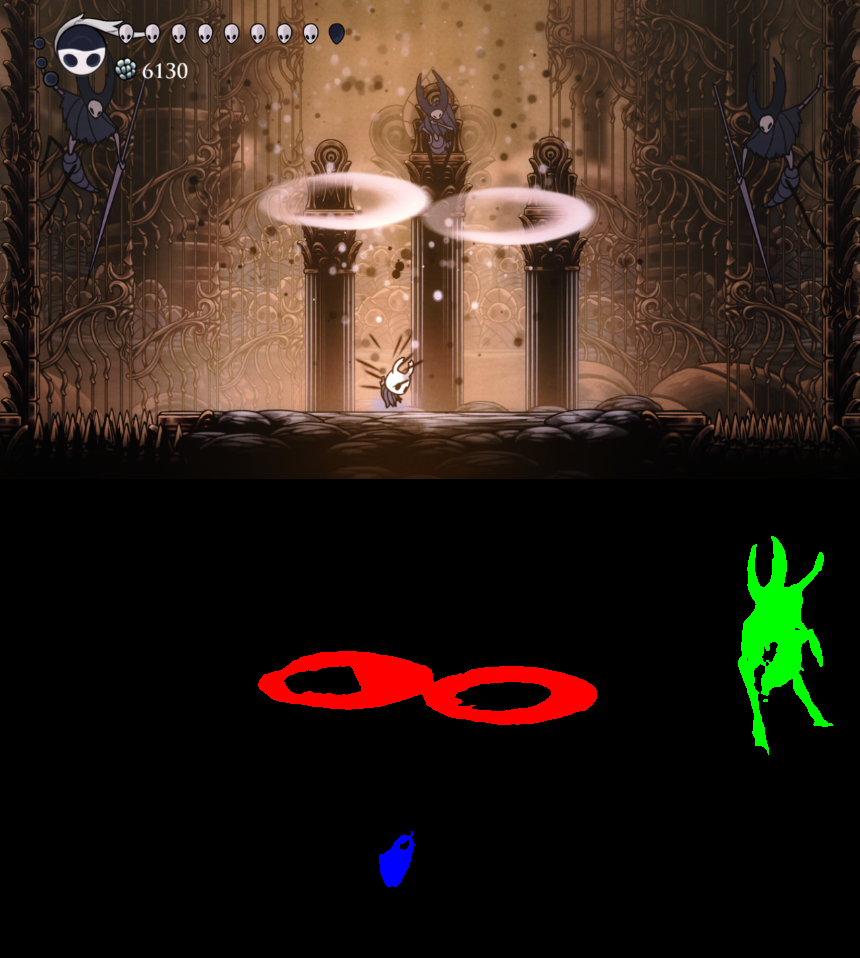
\includegraphics[width=\linewidth]{figures/MantisLords-miss.png}
     \caption{Miss one lord.}
    \end{subfigure}
    \hfill
    \begin{subfigure}[b]{0.4\textwidth}
     \centering
     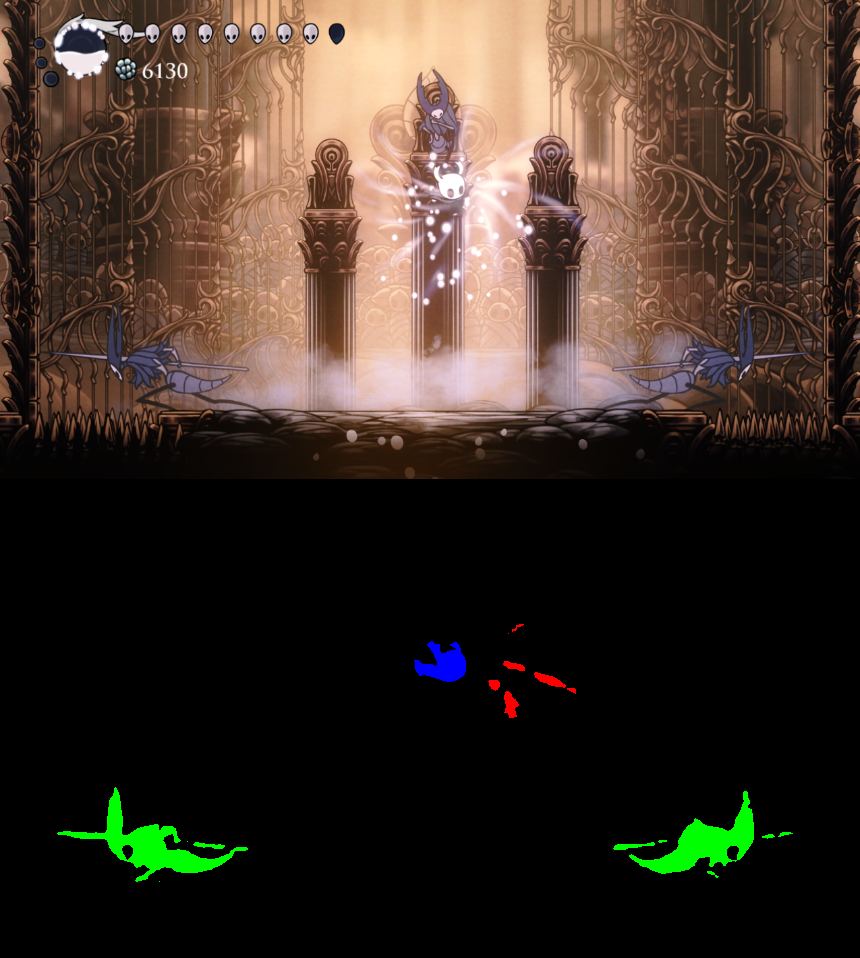
\includegraphics[width=\linewidth]{figures/MantisLords-hit.png}
     \caption{Successfully identify two lords.}
    \end{subfigure}
    }
    \caption{
        Sample frame and segmentation masks generated by Cutie from the Hollow Knight Mantis Lords. 
        Cutie may lose track of one of the lords (represented with green masks).
        This tracking issue is more likely to occur not only in this scenario but also in other environments where duplicated instances are present, compared to scenes with a single instance.
    } \label{fig:MantisLords-miss-hit}
\end{figure} 

\begin{figure}[h]
     \centering
     \resizebox{0.5\textwidth}{!}{
     \begin{subfigure}[b]{0.25\textwidth}
         \centering
         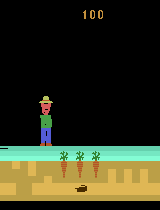
\includegraphics[width=\textwidth]{figures/Gopher-frame.png}
         \caption{Sample frame.}
     \end{subfigure}
     \hfill
     \begin{subfigure}[b]{0.25\textwidth}
         \centering
         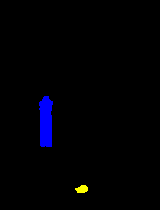
\includegraphics[width=\textwidth]{figures/Gopher-mask.png}
         \caption{Annotation mask.}
     \end{subfigure}
     }
    \caption{
        Sample frame and annotation segmentation masks from Atari Gopher.
        We only specify two objects for Gopher.
        The tunnel in the ground, which is the navigable space for the gopher, is challenging to encode as an object given our model structure.
    } \label{fig:Gopher-frame-mask}
\end{figure} 

\newpage
\section{Sample Annotations for Atari, Hollow Knight, and Metaworld}
Figure \ref{fig:Atari-sample-annotations}, \ref{fig:HollowKnight-sample-annotations}, and \ref{fig:Metaworld-sample-annotations} present sample frames and annotations used by our method in Atari, Hollow Knight, and Metaworld, respectively.
For each task in Atari and Metaworld, we annotate 6 frames, and for each boss in Hollow Knight, we annotate 12 frames.

\begin{figure}[h]
    \centering
    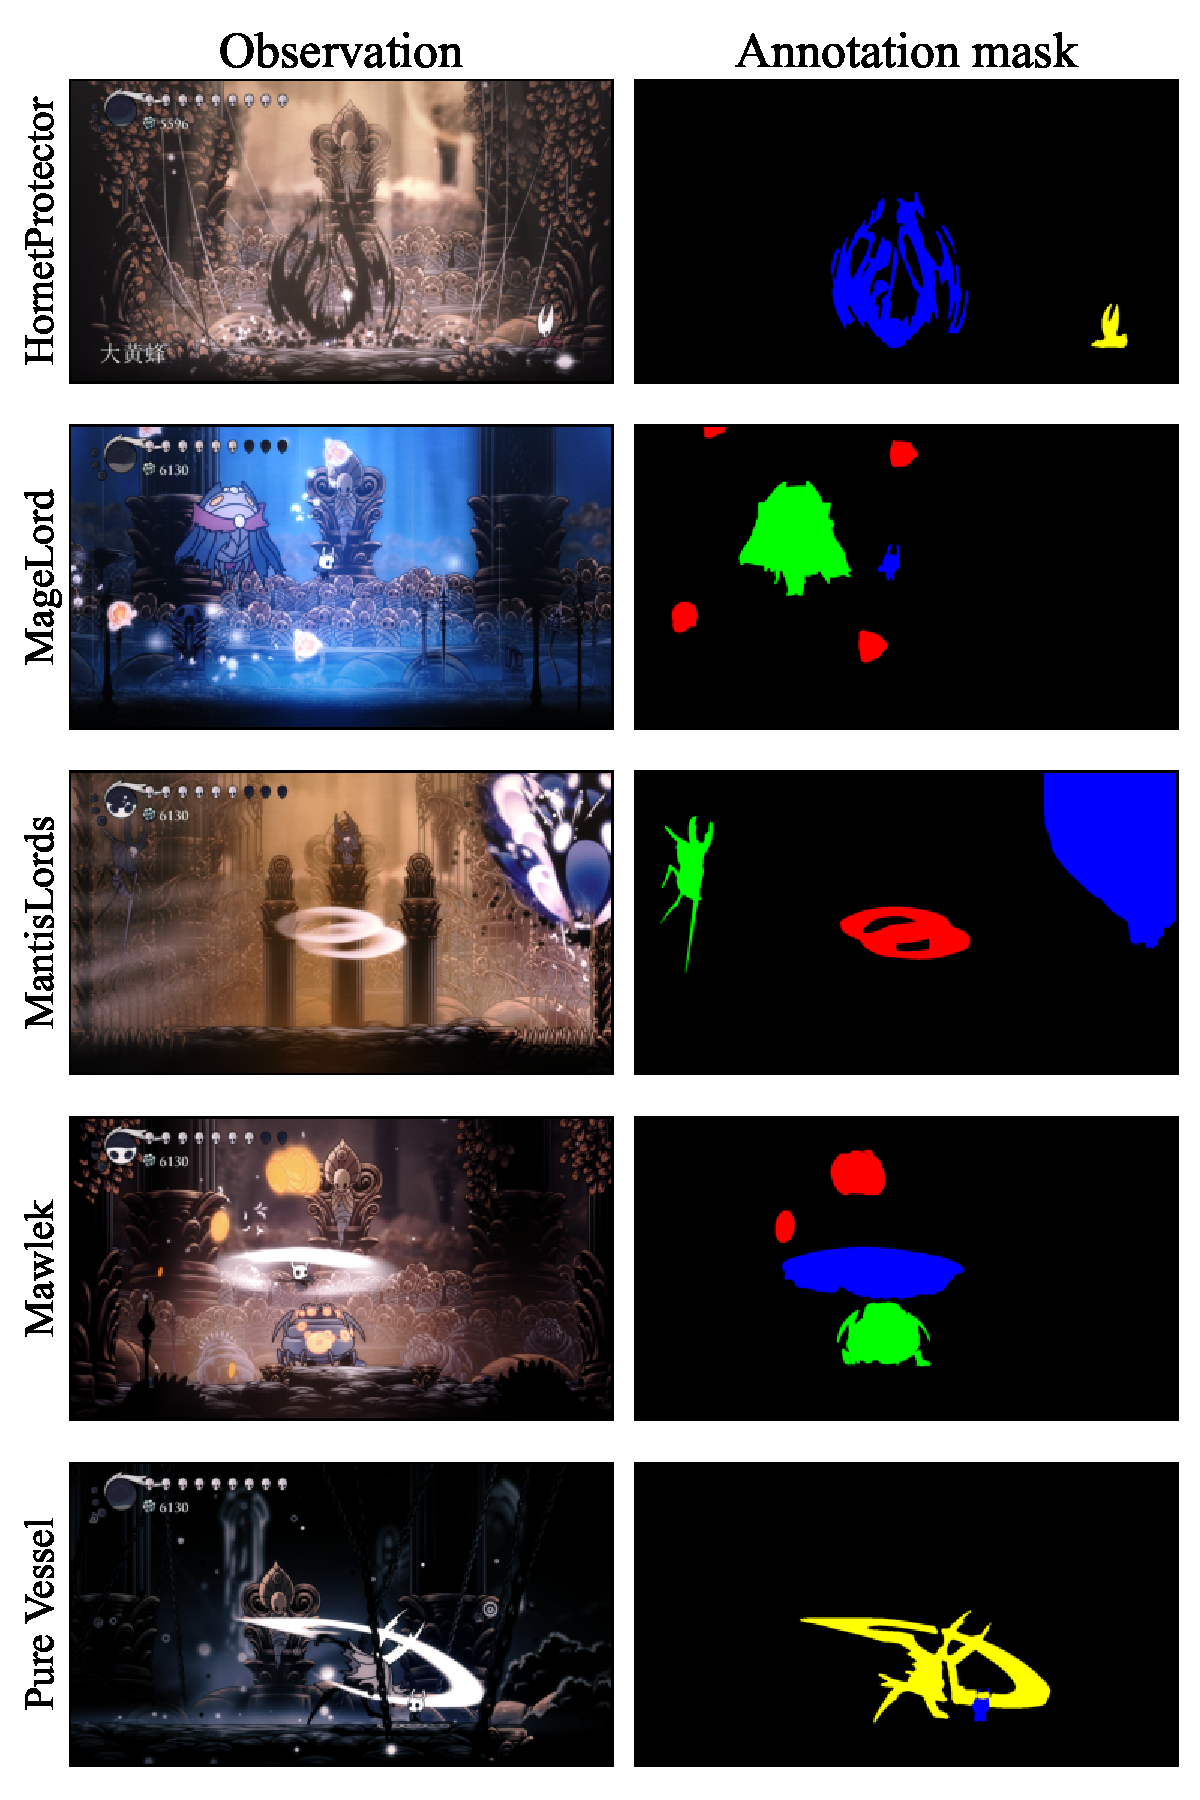
\includegraphics[width=0.5\textwidth]{figures/HollowKnight-sample-annotations.pdf}
    \caption{
        Sample frames and annotation masks for Hollow Knight bosses.
    }
    \label{fig:HollowKnight-sample-annotations}
\end{figure}

\begin{figure}[h]
    \centering
    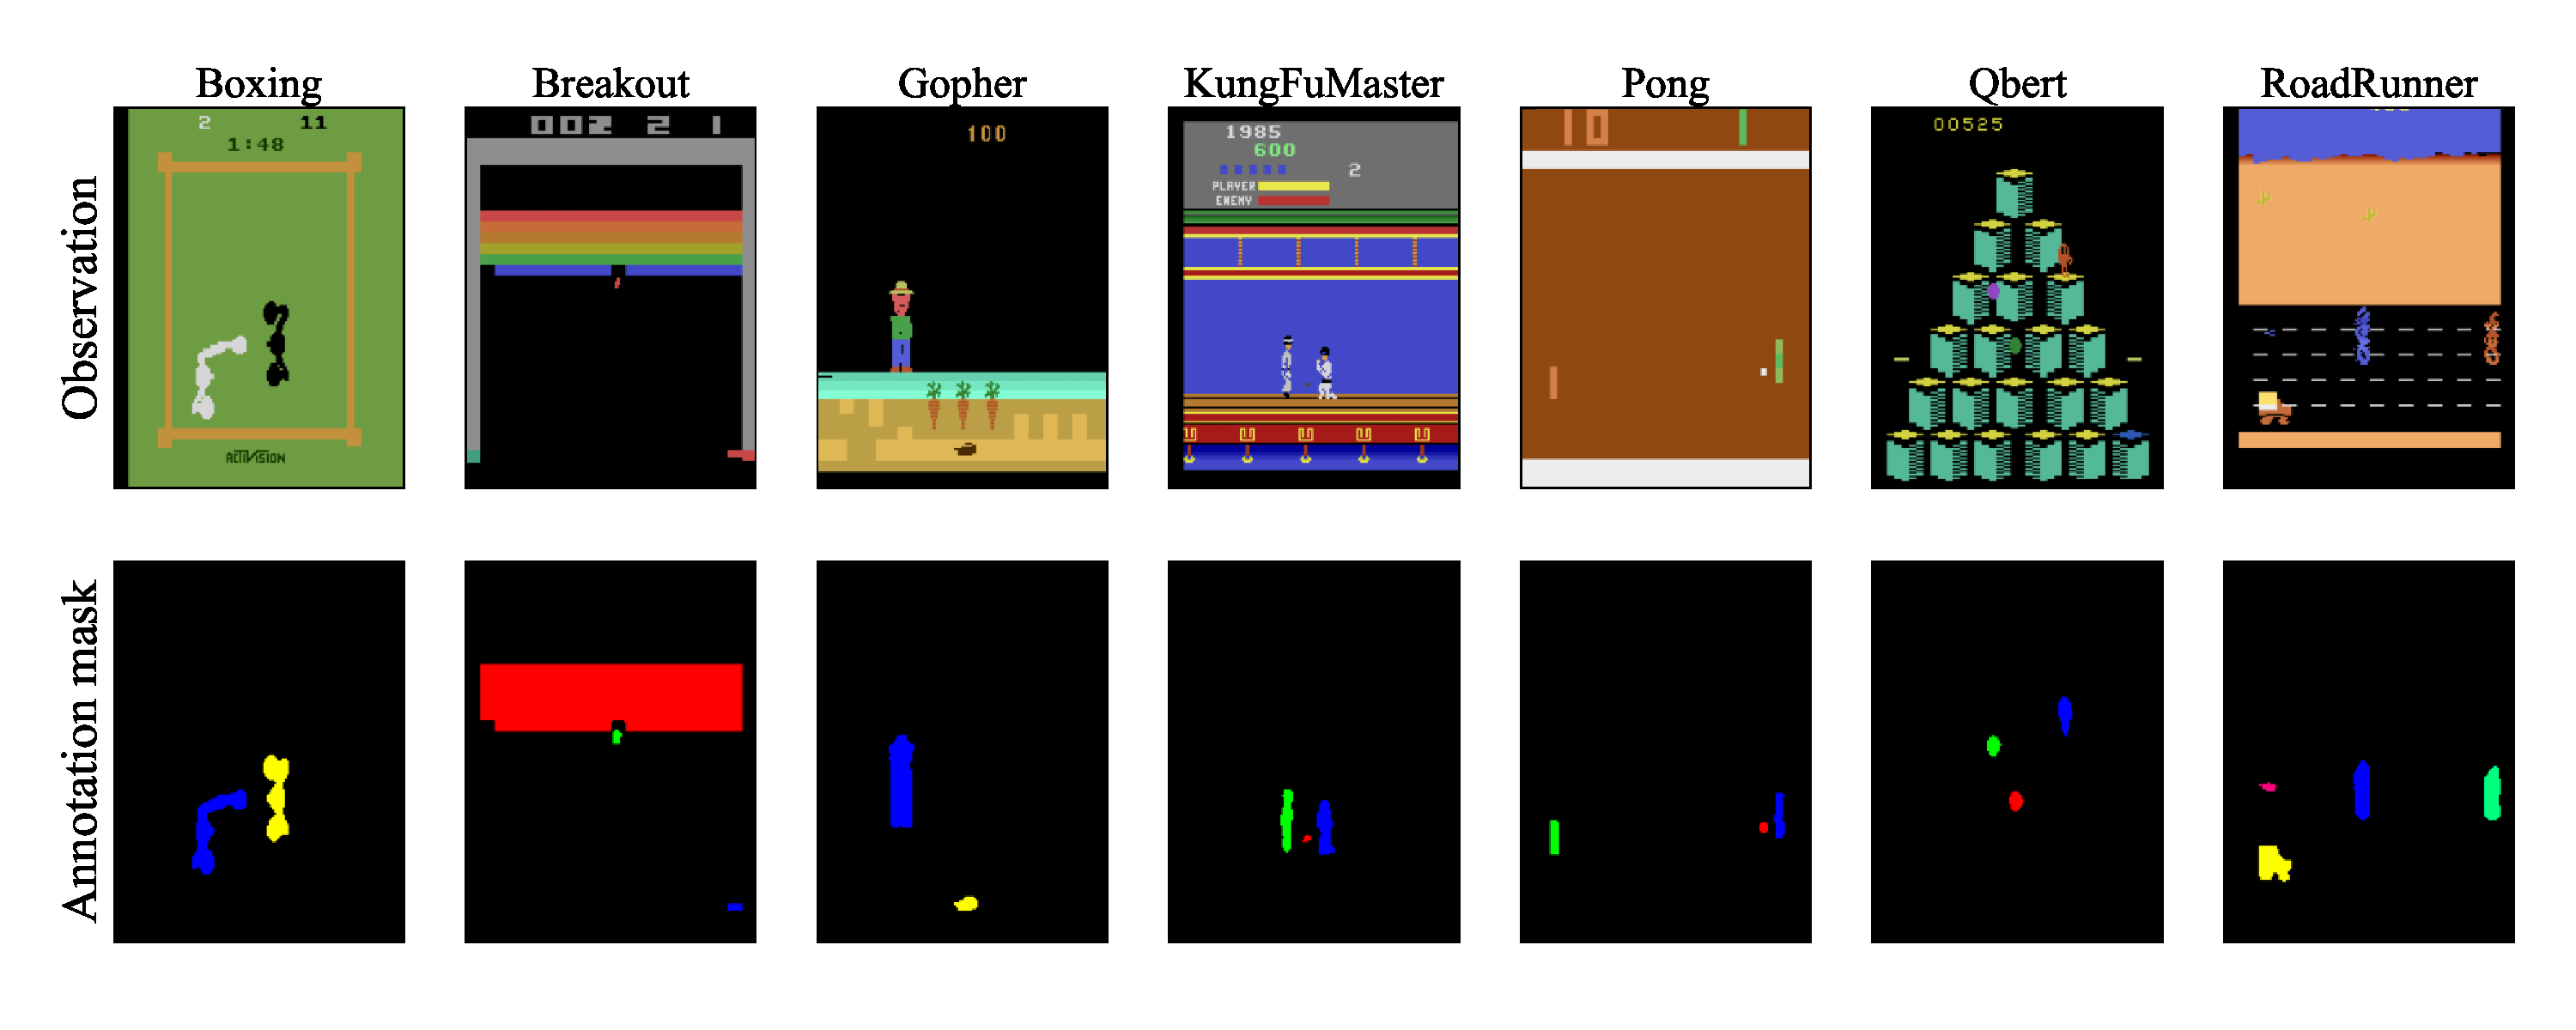
\includegraphics[width=0.9\textwidth]{figures/Atari-sample-annotations.pdf}
    \caption{
        Sample frames and annotation masks for Atari games.
    }
    \label{fig:Atari-sample-annotations}
\end{figure}


\newpage

\begin{figure}[h]
    \centering
    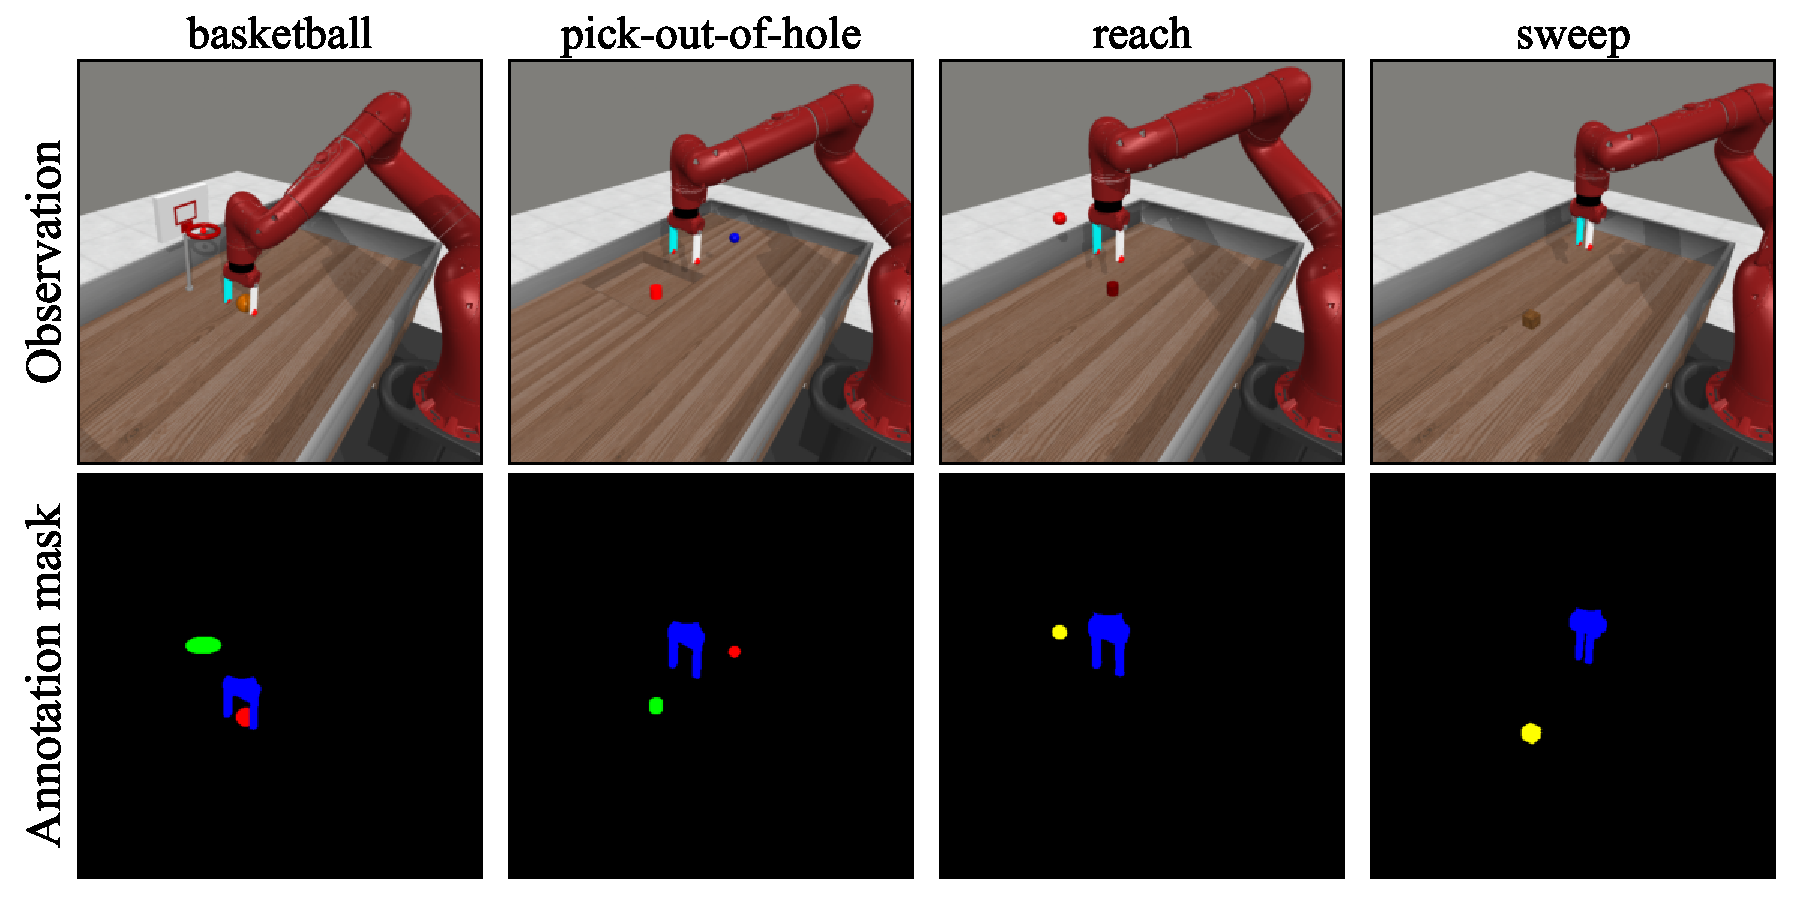
\includegraphics[width=0.6\textwidth]{figures/Metaworld-sample-annotations.pdf}
    \caption{
        Sample frames and annotation masks for Meta-world tasks.
    }
    \label{fig:Metaworld-sample-annotations}
\end{figure}

\section{Ablation on Missing Objects}
We conducted an ablation study on removing annotated objects, and all experiments only use object features with no visual input for the world model.
We found that:
\begin{enumerate}
    \item \textbf{Missing the object that is directly influenced or controlled by the input actions} causes a significant performance drop. Increasing the number of tracked objects generally improves performance.
    \item Some objects (e.g., the brick wall in Breakout) \textbf{may negatively affect performance}. We believe this arises from current video segmentation algorithms’ limited sensitivity to subtle object-level changes (the entire brick wall is treated as a single object). This limitation is discussed in Appendix~\ref{sec:illustration-of-limitations}.
\end{enumerate}

\begin{figure}[h]
    \centering
    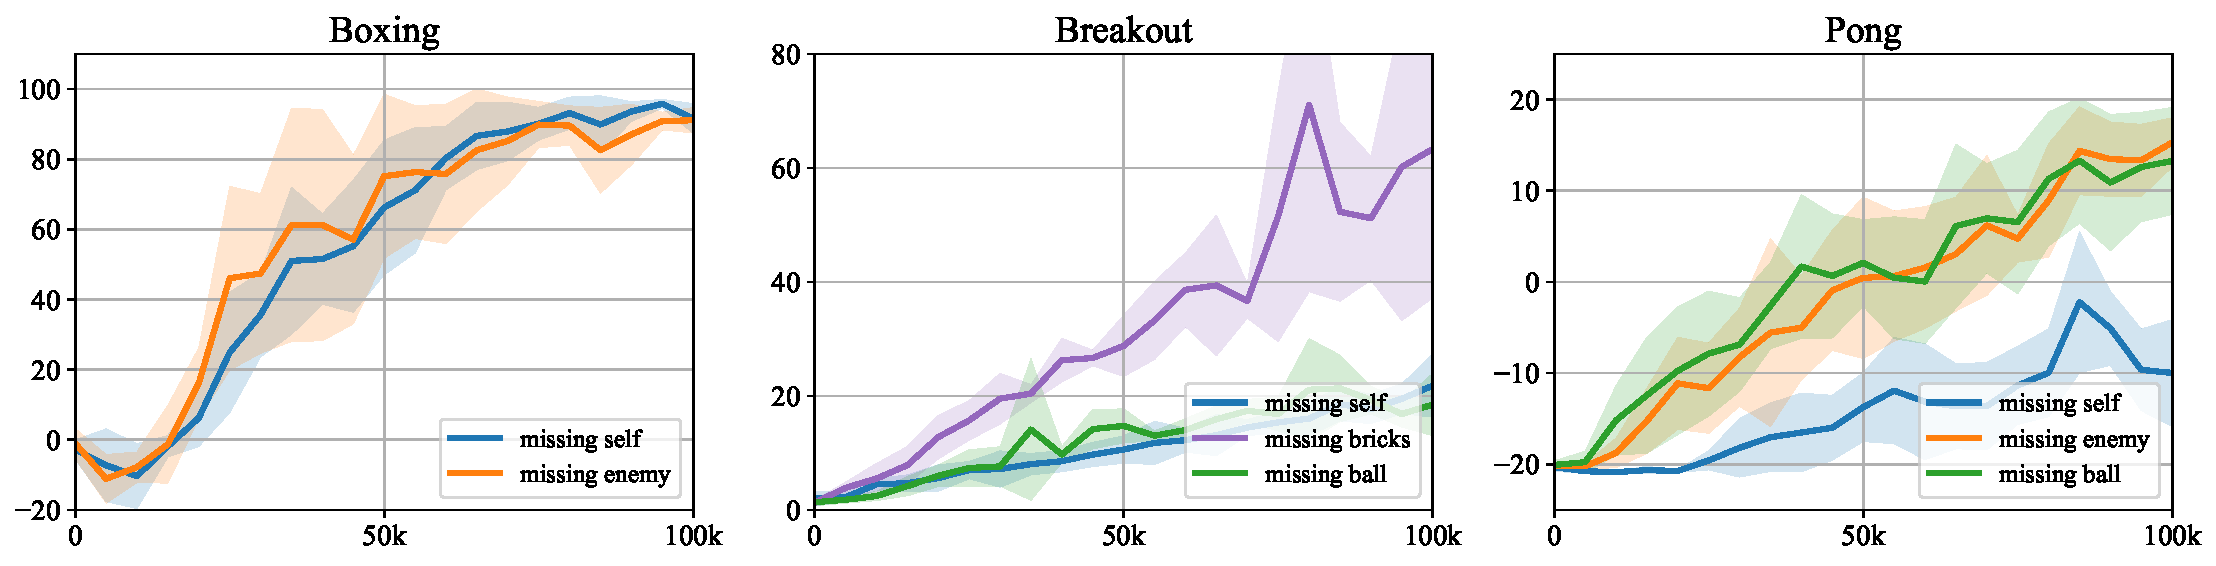
\includegraphics[width=0.85\textwidth]{figures/missing_ablation.pdf}
    \caption{
        Ablation study on missing objects.
        Sample game observations can be found in Figure \ref{fig:Atari-sample-annotations}.
    }
    \label{fig:missing-objects}
\end{figure}

\newpage
\section{Unconditional SAM on Hollow Knight}
At the beginning of our study, we also explored the possibility of performing segmentation using SAM \citep{kirillov_segment_2023, ravi_sam_2024} without any labeled frames.
The results, as illustrated in Figure~\ref{fig:uncon-sam}, show that SAM can roughly distinguish different objects in the Hollow Knight environment; however, the alignment of semantic meaning and the delineation of object scales were not satisfactory in the absence of prompts.
As a result, the quality of the object feature wouldn't be sufficient to support the control objectives of our framework.
These observations motivated us to incorporate targeted supervision into our method design.

\begin{figure}[h]
    \centering
    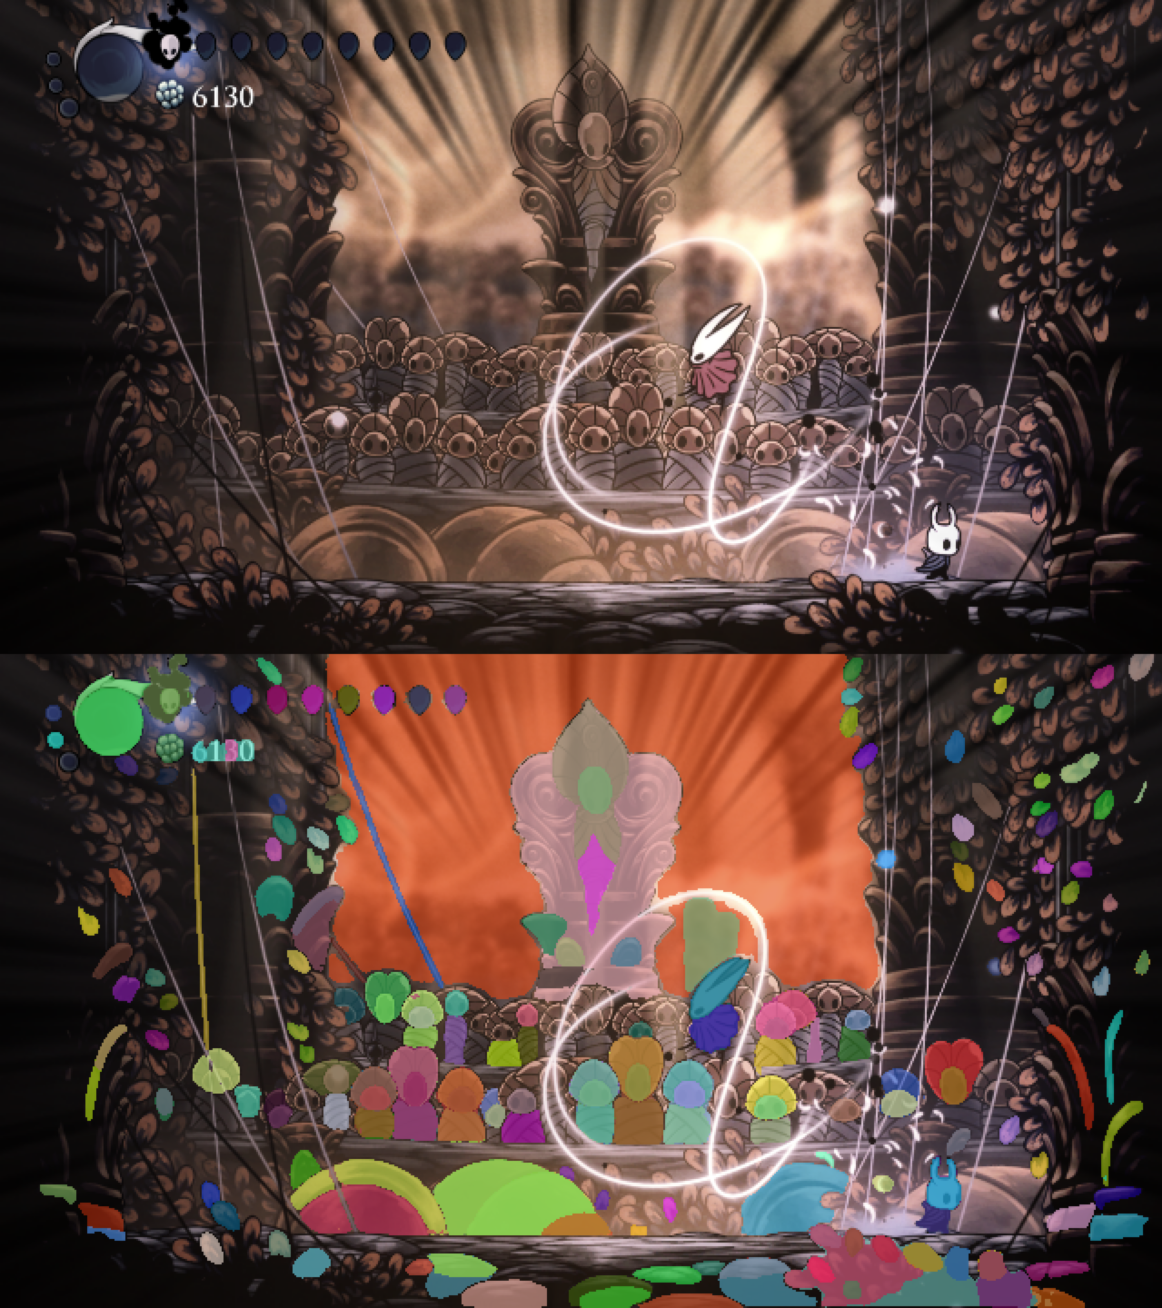
\includegraphics[width=0.6\textwidth]{figures/uncon-sam.png}
    \caption{
        Sample unconditional segmentation results with SAM on Hollow Knight.
    }
    \label{fig:uncon-sam}
\end{figure}

\section{The Use of Large Language Models (LLMs)}
% https://iclr.cc/Conferences/2026/AuthorGuide LLM requirements
We use LLMs for polishing and grammar checking. No content is directly generated with LLMs.